% Practice Test 04 — Virginia Edition
% Questions: 30 (21 MC + 9 SA)
% Generated by scripts/generate_practice_tests.py

\begin{practiceQuestion}{1-4-q06}{mc}
\begin{questionText}
A car travels $55$ miles per hour. Which equation gives the distance $d$ for $t$ hours?
\end{questionText}
\choiceA{$d = t + 55$}
\choiceB{$d = 55t$}
\choiceC{$t = 55d$}
\choiceD{$d = \frac{55}{t}$}
\correctAnswer{B}
\explanation{Distance $=$ rate $\times$ time, so $d = 55t$.}
\end{practiceQuestion}

\begin{practiceQuestion}{2-1-q06}{mc}
\begin{questionText}
$14$ is what percent of $56$?
\end{questionText}
\choiceA{$14\%$}
\choiceB{$20\%$}
\choiceC{$25\%$}
\choiceD{$28\%$}
\correctAnswer{C}
\explanation{Divide the part by the whole: $14 \div 56 = 0.25 = 25\%$.}
\end{practiceQuestion}

\begin{practiceQuestion}{2-2-q04}{mc}
\begin{questionText}
Which proportion shows that $42$ is $60\%$ of some number $w$?
\end{questionText}
\choiceA{$\dfrac{42}{w} = \dfrac{60}{100}$}
\choiceB{$\dfrac{w}{42} = \dfrac{60}{100}$}
\choiceC{$\dfrac{60}{42} = \dfrac{w}{100}$}
\choiceD{$\dfrac{42}{60} = \dfrac{w}{100}$}
\correctAnswer{A}
\explanation{Part ($42$) over whole ($w$) equals percent ($60$) over $100$: $\frac{42}{w} = \frac{60}{100}$.}
\end{practiceQuestion}

\begin{practiceQuestion}{2-3-q11}{mc}
\begin{questionText}
Miranda says that a $50\%$ increase followed by a $50\%$ decrease gives back the original price. Is she correct?
\end{questionText}
\choiceA{Yes, because the two changes cancel out}
\choiceB{No, the result is less than the original}
\choiceC{No, the result is more than the original}
\choiceD{It depends on the starting price}
\correctAnswer{B}
\explanation{Start with $\$100$. Increase $50\%$: $\$150$. Decrease $50\%$: $150 \times 0.50 = \$75$. That is less than $\$100$.}
\end{practiceQuestion}

\begin{practiceQuestion}{2-7-q13}{mc}
\begin{questionText}
A student estimated a hallway was $60$ meters long. The actual length was $50$ meters. What is the percent error?
\end{questionText}
\choiceA{$10\%$}
\choiceB{$16.7\%$}
\choiceC{$20\%$}
\choiceD{$25\%$}
\correctAnswer{C}
\explanation{$\frac{|60-50|}{50} \times 100 = \frac{10}{50} \times 100 = 20\%$.}
\end{practiceQuestion}

\begin{practiceQuestion}{3-2-q24}{sa}
\begin{questionText}
A football team has the following plays: gain $7$ yards, lose $3$ yards, lose $5$ yards, gain $2$ yards. What is the net yardage?
\end{questionText}
\correctAnswer{$1$ yard}
\explanation{$7 + (-3) + (-5) + 2 = 1$. Gains: $7 + 2 = 9$. Losses: $3 + 5 = 8$. Net: $9 - 8 = 1$ yard gained.}
\end{practiceQuestion}

\begin{practiceQuestion}{3-3-q28}{gmc}
\begin{questionText}
The table shows daily high temperatures for a city.

\begin{center}
\begin{tabular}{|c|c|}
\hline
\textbf{Day} & \textbf{High Temp (°F)} \\
\hline
Monday & $-3$ \\
\hline
Tuesday & $8$ \\
\hline
Wednesday & $-5$ \\
\hline
\end{tabular}
\end{center}

What is the difference between Tuesday's and Wednesday's temperatures?
\end{questionText}
\choiceA{$3°$F}
\choiceB{$-3°$F}
\choiceC{$13°$F}
\choiceD{$-13°$F}
\correctAnswer{C}
\explanation{$8 - (-5) = 8 + 5 = 13°$F.}
\end{practiceQuestion}

\begin{practiceQuestion}{3-4-q25}{sa}
\begin{questionText}
A recipe calls for $1\dfrac{3}{4}$ cups of flour. You already added $\dfrac{5}{8}$ cup. How much more flour do you need?
\end{questionText}
\correctAnswer{$1\dfrac{1}{8}$ cups}
\explanation{$1\frac{3}{4} - \frac{5}{8} = \frac{7}{4} - \frac{5}{8} = \frac{14}{8} - \frac{5}{8} = \frac{9}{8} = 1\frac{1}{8}$ cups.}
\end{practiceQuestion}

\begin{practiceQuestion}{4-3-q02}{mc}
\begin{questionText}
Expand $5(2a - 3)$.
\end{questionText}
\choiceA{$10a - 3$}
\choiceB{$7a - 3$}
\choiceC{$10a - 15$}
\choiceD{$10a + 15$}
\correctAnswer{C}
\explanation{$5 \times 2a = 10a$ and $5 \times (-3) = -15$. Result: $10a - 15$.}
\end{practiceQuestion}

\begin{practiceQuestion}{4-4-q27}{gmc}
\begin{questionText}
The arrays below show how $12$ tiles can be arranged. Which arrangement shows that $12 = 4 \times 3$?

\begin{center}
\begin{tikzpicture}[scale=0.5]
  % Arrangement A: 2 x 6
  \node[font=\bfseries] at (3, 3.5) {A: $2 \times 6$};
  \foreach \x in {0,...,5} {
    \foreach \y in {0,...,1} {
      \fill[funBlue!40] (\x+0.1, \y+0.1) rectangle (\x+0.9, \y+0.9);
      \draw[thick] (\x+0.1, \y+0.1) rectangle (\x+0.9, \y+0.9);
    }
  }
  % Arrangement B: 4 x 3
  \begin{scope}[xshift=8cm]
  \node[font=\bfseries] at (1.5, 5) {B: $4 \times 3$};
  \foreach \x in {0,...,2} {
    \foreach \y in {0,...,3} {
      \fill[funGreen!40] (\x+0.1, \y+0.1) rectangle (\x+0.9, \y+0.9);
      \draw[thick] (\x+0.1, \y+0.1) rectangle (\x+0.9, \y+0.9);
    }
  }
  \end{scope}
  % Arrangement C: 1 x 12
  \begin{scope}[xshift=13cm]
  \node[font=\bfseries] at (6, 1.5) {C: $1 \times 12$};
  \foreach \x in {0,...,11} {
    \fill[funOrange!40] (\x+0.1, 0.1) rectangle (\x+0.9, 0.9);
    \draw[thick] (\x+0.1, 0.1) rectangle (\x+0.9, 0.9);
  }
  \end{scope}
\end{tikzpicture}
\end{center}
\end{questionText}
\choiceA{Arrangement A}
\choiceB{Arrangement B}
\choiceC{Arrangement C}
\choiceD{All three arrangements}
\correctAnswer{B}
\explanation{Arrangement B shows $4$ rows and $3$ columns, illustrating $12 = 4 \times 3$. This connects to factoring: $12$ can be written as the product $4(3)$.}
\end{practiceQuestion}

\begin{practiceQuestion}{5-4-q05}{mc}
\begin{questionText}
Solve $\dfrac{2x}{5} - 1 = 3$.
\end{questionText}
\choiceA{$x = 5$}
\choiceB{$x = 10$}
\choiceC{$x = 4$}
\choiceD{$x = 20$}
\correctAnswer{B}
\explanation{Add $1$: $\frac{2x}{5} = 4$. Multiply by $5$: $2x = 20$. Divide by $2$: $x = 10$. Check: $\frac{2(10)}{5} - 1 = 4 - 1 = 3$ \checkmark.}
\end{practiceQuestion}

\begin{practiceQuestion}{5-5-q29}{gsa}
\begin{questionText}
The balance scale tips to the left. Write and solve the inequality that describes this situation.

\begin{center}
\begin{tikzpicture}[scale=0.7]
  % Tilted beam (left side heavier)
  \draw[thick] (0,-0.5) -- (-0.4,-1.2) -- (0.4,-1.2) -- cycle;
  \draw[thick] (-4.5,0.5) -- (4.5,-0.5);
  % Left pan (lower = heavier)
  \draw[thick] (-4.5,0.5) -- (-5.3,0) -- (-3.7,0) -- (-4.5,0.5);
  \draw[thick,fill=funBlue!20] (-5.3,0) -- (-5.3,-0.4) -- (-3.7,-0.4) -- (-3.7,0) -- cycle;
  \node at (-4.5,-0.2) {$2x + 8$};
  % Right pan (higher = lighter)
  \draw[thick] (4.5,-0.5) -- (5.3,-1) -- (3.7,-1) -- (4.5,-0.5);
  \draw[thick,fill=funOrange!20] (3.7,-1) -- (3.7,-1.4) -- (5.3,-1.4) -- (5.3,-1) -- cycle;
  \node at (4.5,-1.2) {$20$};
\end{tikzpicture}
\end{center}
\end{questionText}
\correctAnswer{$2x + 8 > 20$; $x > 6$}
\explanation{The left side is heavier (tips down), so $2x + 8 > 20$. Subtract $8$: $2x > 12$. Divide by $2$: $x > 6$.}
\end{practiceQuestion}

\begin{practiceQuestion}{5-6-q26}{gmc}
\begin{questionText}
Which inequality matches the graph below?

\begin{center}
\begin{tikzpicture}[scale=0.7]
  \draw[thick,->] (-5,0) -- (5,0);
  \foreach \x in {-4,...,4} \draw (\x,0.15) -- (\x,-0.15) node[below] {$\x$};
  \draw[thick,funBlue,<-] (-5,0) -- (1,0);
  \fill[funBlue] (1,0) circle (4pt);
\end{tikzpicture}
\end{center}
\end{questionText}
\choiceA{$x \leq 1$}
\choiceB{$x < 1$}
\choiceC{$x \geq 1$}
\choiceD{$x > 1$}
\correctAnswer{A}
\explanation{Closed circle at $1$ with shading to the left means $x \leq 1$.}
\end{practiceQuestion}

\begin{practiceQuestion}{6-1-q13}{mc}
\begin{questionText}
A floor plan uses the scale $1$ cm $= 2$ m. A closet measures $1.5$ cm by $1$ cm on the plan. What is the actual area?
\end{questionText}
\choiceA{$1.5$ m$^2$}
\choiceB{$3$ m$^2$}
\choiceC{$6$ m$^2$}
\choiceD{$12$ m$^2$}
\correctAnswer{C}
\explanation{Actual dimensions: $1.5 \times 2 = 3$ m and $1 \times 2 = 2$ m. Area: $3 \times 2 = 6$ m$^2$.}
\end{practiceQuestion}

\begin{practiceQuestion}{6-2-q13}{mc}
\begin{questionText}
A drawing uses $1$ cm $= 6$ m. It is redrawn at $1$ cm $= 2$ m. The original drawing is $8$ cm by $5$ cm. What is the perimeter of the new drawing?
\end{questionText}
\choiceA{$26$ cm}
\choiceB{$39$ cm}
\choiceC{$78$ cm}
\choiceD{$120$ cm}
\correctAnswer{C}
\explanation{Scale ratio: $\frac{6}{2} = 3$. New dimensions: $8 \times 3 = 24$ cm and $5 \times 3 = 15$ cm. New perimeter: $2(24 + 15) = 78$ cm.}
\end{practiceQuestion}

\begin{practiceQuestion}{6-5-q15}{mc}
\begin{questionText}
A pyramid with a square base is sliced with a horizontal cut near the top. What shape is the cross-section?
\end{questionText}
\choiceA{A very small square}
\choiceB{A triangle}
\choiceC{A point}
\choiceD{A circle}
\correctAnswer{A}
\explanation{A horizontal cut of a square pyramid parallel to the base gives a square. Near the top, the square is very small. At the very apex it would be a point, but a cut ``near the top'' gives a small square.}
\end{practiceQuestion}

\begin{practiceQuestion}{6-6-q19}{sa}
\begin{questionText}
Find the complement of $67°$.
\end{questionText}
\correctAnswer{$23°$}
\explanation{$90° - 67° = 23°$.}
\end{practiceQuestion}

\begin{practiceQuestion}{6-7-q27}{gmc}
\begin{questionText}
Point $T$ is shown on the coordinate plane. It is translated right $3$ and up $4$. Where is $T'$?

\begin{center}
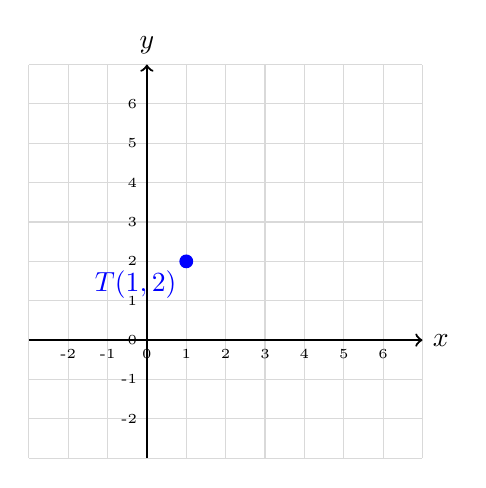
\begin{tikzpicture}[scale=0.5]
  \draw[step=1,gray!30,thin] (-3,-3) grid (7,7);
  \draw[thick,->] (-3,0) -- (7,0) node[right]{$x$};
  \draw[thick,->] (0,-3) -- (0,7) node[above]{$y$};
  \fill[blue] (1,2) circle (5pt);
  \node[below left,blue] at (1,2) {$T(1,2)$};
  \foreach \x in {-2,...,6} \node[below,font=\tiny] at (\x,0) {\x};
  \foreach \y in {-2,...,6} \node[left,font=\tiny] at (0,\y) {\y};
\end{tikzpicture}
\end{center}
\end{questionText}
\choiceA{$(4, 6)$}
\choiceB{$(4, -2)$}
\choiceC{$(-2, 6)$}
\choiceD{$(1, 6)$}
\correctAnswer{A}
\explanation{Right $3$: $1 + 3 = 4$. Up $4$: $2 + 4 = 6$. So $T'(4, 6)$.}
\end{practiceQuestion}

\begin{practiceQuestion}{6-8-q24}{sa}
\begin{questionText}
Two similar triangles have corresponding sides $6$ and $10$. If the perimeter of the smaller triangle is $18$ cm, what is the perimeter of the larger triangle?
\end{questionText}
\correctAnswer{$30$ cm}
\explanation{Scale factor: $\frac{10}{6} = \frac{5}{3}$. Larger perimeter: $18 \times \frac{5}{3} = 30$ cm.}
\end{practiceQuestion}

\begin{practiceQuestion}{7-4-q01}{mc}
\begin{questionText}
A composite shape is made of a rectangle that is $10$ cm by $4$ cm and a triangle with base $10$ cm and height $3$ cm attached to one side. What is the total area?
\end{questionText}
\choiceA{$40$ cm$^2$}
\choiceB{$55$ cm$^2$}
\choiceC{$70$ cm$^2$}
\choiceD{$120$ cm$^2$}
\correctAnswer{B}
\explanation{Rectangle: $10 \times 4 = 40$ cm$^2$. Triangle: $\frac{1}{2} \times 10 \times 3 = 15$ cm$^2$. Total: $40 + 15 = 55$ cm$^2$.}
\end{practiceQuestion}

\begin{practiceQuestion}{7-5-q02}{mc}
\begin{questionText}
What is the surface area of a rectangular prism with length $5$ cm, width $3$ cm, and height $2$ cm?
\end{questionText}
\choiceA{$30$ cm$^2$}
\choiceB{$62$ cm$^2$}
\choiceC{$46$ cm$^2$}
\choiceD{$31$ cm$^2$}
\correctAnswer{B}
\explanation{$SA = 2(5 \times 3) + 2(5 \times 2) + 2(3 \times 2) = 30 + 20 + 12 = 62$ cm$^2$.}
\end{practiceQuestion}

\begin{practiceQuestion}{7-6-q15}{mc}
\begin{questionText}
A sandbox is $6$ ft long, $4$ ft wide, and $1$ ft deep. Sand costs \$$2$ per cubic foot. How much does it cost to fill the sandbox?
\end{questionText}
\choiceA{$\$12$}
\choiceB{$\$24$}
\choiceC{$\$48$}
\choiceD{$\$96$}
\correctAnswer{C}
\explanation{$V = 6 \times 4 \times 1 = 24$ ft$^3$. Cost: $24 \times 2 = \$48$.}
\end{practiceQuestion}

\begin{practiceQuestion}{7-7-q21}{sa}
\begin{questionText}
Find the surface area of a cylinder with radius $4$ cm and height $9$ cm. Use $\pi \approx 3.14$.
\end{questionText}
\correctAnswer{$326.56$ cm$^2$}
\explanation{$SA = 2\pi r^2 + 2\pi rh = 2(3.14)(16) + 2(3.14)(4)(9) = 100.48 + 226.08 = 326.56$ cm$^2$.}
\end{practiceQuestion}

\begin{practiceQuestion}{8-1-q03}{mc}
\begin{questionText}
Which sampling method is most likely to produce a representative sample of a school's students?
\end{questionText}
\choiceA{Survey students in the cafeteria during lunch}
\choiceB{Survey every fifth student on an alphabetical class list}
\choiceC{Survey students who volunteer to participate}
\choiceD{Survey only students in honors classes}
\correctAnswer{B}
\explanation{Selecting every fifth student from a list is systematic and gives all students an equal chance, making it more representative.}
\end{practiceQuestion}

\begin{practiceQuestion}{8-3-q21}{sa}
\begin{questionText}
Data set: $4, 6, 7, 8, 10$. The mean is $7$. Find the MAD.
\end{questionText}
\correctAnswer{$1.6$}
\explanation{Deviations from mean: $|4-7|+|6-7|+|7-7|+|8-7|+|10-7| = 3+1+0+1+3 = 8$. MAD $= \frac{8}{5} = 1.6$.}
\end{practiceQuestion}

\begin{practiceQuestion}{8-4-q24}{sa}
\begin{questionText}
Explain one advantage of using IQR instead of range to describe the spread of a data set.
\end{questionText}
\correctAnswer{IQR is not affected by outliers}
\explanation{Range uses only the extreme values, which can be misleading with outliers. IQR measures the middle $50\%$ and gives a more stable picture of typical variability.}
\end{practiceQuestion}

\begin{practiceQuestion}{8-5-q17}{mc}
\begin{questionText}
A student reads $4 \mid 7$ from a stem-and-leaf plot and says the value is $74$. What did the student do wrong?
\end{questionText}
\choiceA{The student added the digits}
\choiceB{The student reversed the stem and leaf}
\choiceC{The student multiplied the digits}
\choiceD{Nothing — $74$ is correct}
\correctAnswer{B}
\explanation{$4 \mid 7$ means the stem ($4$) is the tens digit and the leaf ($7$) is the ones digit, so it represents $47$, not $74$.}
\end{practiceQuestion}

\begin{practiceQuestion}{9-3-q10}{mc}
\begin{questionText}
In $100$ spins of a spinner, red appears $22$ times, blue appears $48$ times, and green appears $30$ times. Which color has an experimental probability closest to $\frac{1}{2}$?
\end{questionText}
\choiceA{Red}
\choiceB{Blue}
\choiceC{Green}
\choiceD{Red and Green are equally close}
\correctAnswer{B}
\explanation{Blue: $\frac{48}{100} = 0.48$, which is closest to $0.50$.}
\end{practiceQuestion}

\begin{practiceQuestion}{9-6-q19}{sa}
\begin{questionText}
Two dice are rolled. What is the probability that the sum is $10$ or greater? Write your answer as a fraction in simplest form.
\end{questionText}
\correctAnswer{$\frac{1}{6}$}
\explanation{Sum $10$: $(4,6), (5,5), (6,4)$ — $3$ outcomes. Sum $11$: $(5,6), (6,5)$ — $2$. Sum $12$: $(6,6)$ — $1$. Total: $6$ out of $36$. $P = \frac{6}{36} = \frac{1}{6}$.}
\end{practiceQuestion}

\begin{practiceQuestion}{9-7-q28}{gmc}
\begin{questionText}
The table shows a simulation using random digits $0$--$9$ to model a $30\%$ chance of rain. Digits $0$, $1$, $2$ represent rain. Based on the $10$ trials below, what is the experimental probability of rain?

\begin{center}
\begin{tabular}{|c|c|c|}
\hline
\textbf{Trial} & \textbf{Digit} & \textbf{Rain?} \\
\hline
$1$ & $5$ & No \\
\hline
$2$ & $1$ & Yes \\
\hline
$3$ & $8$ & No \\
\hline
$4$ & $0$ & Yes \\
\hline
$5$ & $3$ & No \\
\hline
$6$ & $7$ & No \\
\hline
$7$ & $2$ & Yes \\
\hline
$8$ & $9$ & No \\
\hline
$9$ & $4$ & No \\
\hline
$10$ & $6$ & No \\
\hline
\end{tabular}
\end{center}
\end{questionText}
\choiceA{$\frac{2}{10} = 0.20$}
\choiceB{$\frac{3}{10} = 0.30$}
\choiceC{$\frac{4}{10} = 0.40$}
\choiceD{$\frac{7}{10} = 0.70$}
\correctAnswer{B}
\explanation{Rain occurred in trials $2$, $4$, and $7$ — that is $3$ out of $10$. $P = \frac{3}{10} = 0.30$.}
\end{practiceQuestion}
